\documentclass{article}

\usepackage{amsmath, mathrsfs, amssymb, stmaryrd, cancel, relsize,tikz,amsthm}

\theoremstyle{plain}
\newtheorem{theorem}{Theorem}[section]{\bfseries}{\itshape}
\newtheorem{proposition}[theorem]{Proposition}{\bfseries}{\itshape}
\newtheorem{definition}[theorem]{Definition}{\bfseries}{\upshape}
\newtheorem{lemma}[theorem]{Lemma}{\bfseries}{\upshape}
\newtheorem{example}[theorem]{Example}{\bfseries}{\upshape}
\newtheorem{corollary}[theorem]{Corollary}{\bfseries}{\upshape}
\newtheorem{exercise}[theorem]{Exercise}{\bfseries}{\upshape}

\newcommand{\tvs}{\textvisiblespace}
\newcommand{\ra}{\rightarrow}
\newcommand{\la}{\leftarrow}

%\pagenumbering{gobble}

\title{ITCS 532 Foundations of Computer Science\\
Class 1 - Models of Computation}
\author{Rob Egrot}
\date{}

\begin{document}
\maketitle
\subsection{A very brief history of computer science}
In 1928, the mathematician David Hilbert asked whether there exists an algorithm that, given a set $\Gamma$ of first-order sentences, and another first-order sentence $\phi$, will determine whether or not $\phi$ is a logical consequence of $\Gamma$ (i.e. if $\Gamma\models \phi$). Except he didn't exactly, because the concept of an \emph{algorithm} did not exist as it does today. What Hilbert asked (in German) was whether there was some well defined procedure that would take as input the information of $\Gamma$ and $\phi$ and produce the correct answer. This is a difficult question, and part of the difficulty comes from the fact that it is far from clear what it means for something to be a `well defined procedure'. Though mechanical `reasoning' machines had been created at least as far back the 17th century, a formal theory of computation did not yet exist.  

In 1936 the mathematicians Alan Turing and Alonzo Church independently came up with the solution, which turned out to be `no'. For their answers, Turing and Church first had to formalize the concept of a well defined procedure (what we know call an algorithm, after the 9th century Arab mathematician and astronomer Muhammad ibn Musa al-Khwarizmi), and indeed, the concept of \emph{computation} itself. Their formulations appeared at first to be very different, though later they were proved to be equivalent. The point is that both Turing and Church were able to show that, according to their versions of computability, there was no algorithm that would do what Hilbert wanted.

This is interesting mathematics in itself, but more significantly for people not fascinated by formal logic (which is most people), the work done by Turing and Church in this period laid the foundation for the development of computers as we understand them today. In this course we will develop the concept of computation as introduced by Turing. We will explore the limits of computability, and we will ultimately see why Hilbert's question has a negative answer. Later, we will also start to take the running times of algorithms seriously, because, in the real world, an algorithm that solves a problem but takes a billion years to run is not very useful. Before that, we have to start at the beginning, so in this section we will introduce the fundamental concepts of Turing machines and decision problems. 

\subsection{Finite State Machines}
A finite state machine (FSM), also know as a \emph{finite automaton}, is an abstract machine capable of reacting to external inputs in a simple way. At any moment an FSM is in one of a finite number of possible states. The state can change in response to input, and the changing of states is governed by a set of deterministic rules. Formally a finite state machine $M$ is composed of five things:
\begin{enumerate}
\item A finite set of states $Q$.
\item A distinguished set $H\subseteq Q$. This set contains the \emph{halting} states of $M$. If the machine gets to a state in $H$ then it stops running. 
\item A special starting state $q_0\in Q$.
\item A finite set of possible inputs $\Sigma$ sometimes called the \emph{alphabet} of $M$.
\item A function $\delta:(Q\setminus H)\times \Sigma\to Q$. This function controls state change. I.e. $\delta(q,\sigma)=r$ means \emph{if in state $q$ go to state $r$ when receiving input $\sigma$}.
\end{enumerate} 

$\delta$ is sometimes called the \emph{transition function}. Unfortunately different authors sometimes use slightly different definitions. For example, some people let the function $\delta$ be \emph{partial}, that is, they allow it to be undefined for some values of $Q$ and $\Sigma$. What this means is that there has to be a rule for dealing with computations that \emph{hang}, i.e. that reach a point where the next step is undefined. We're not going to worry about this right now, so we just demand that $\delta$ is always \emph{total}, i.e. that it is defined everywhere.

Real world implementations of FSMs are very common. For example, vending machines, ticket machines, turnstiles, some functions of ATMs, automatic lighting systems, and many more! All these run on FSM logic. In the real world FSMs usually respond to input from external sources, e.g. people pressing buttons. 

Now, in the real world people don't always use machines correctly. They might press some buttons then just walk away. There may be arbitrarily long gaps between inputs. A real system has to have a way to deal with this (for example it may have an internal timer that resets the system to the start state after a certain amount of time without receiving any input). This is a problem for engineers to deal with. We're going to abstract this away by ignoring time completely and assuming that the instructions an FSM receives come in an ordered sequence. Since the set of possible inputs is represented by symbols from $\Sigma$, this (finite) ordered sequence is just a finite string from $\Sigma$ (this is why we call $\Sigma$ the alphabet). So an FSM defines a function from the set of all finite strings from $\Sigma$ (we use the notation $\Sigma^*$ to represent this set of finite strings) to the set of states $Q$. The \emph{output} of an FSM (if it has one) is just the final state of a computation that ends in one of the halting states.

\begin{example}
This FSM looks for the sequence $abc$ inside strings composed of letters from the alphabet $\Sigma=\{a,b,c\}$. The circles represent states and the arrows represent transitions based on inputs. The initial state is labeled by $q_0$ and the accept state is marked by a double circle.
\begin{center}
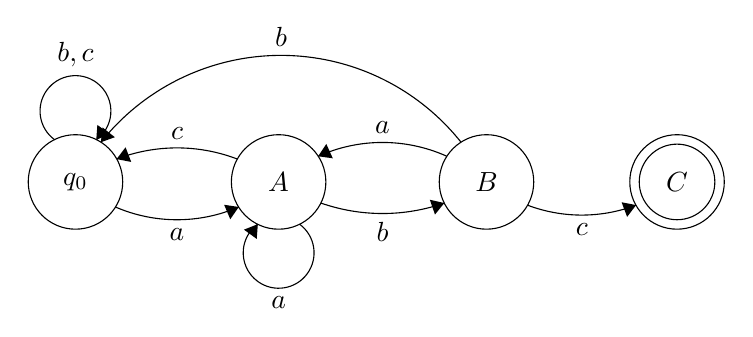
\begin{tikzpicture}[scale=0.2]
\tikzstyle{every node}+=[inner sep=0pt]
\draw [black] (16.6,-30.5) circle (3);
\draw (16.6,-30.5) node {$q_0$};
\draw [black] (29.5,-30.5) circle (3);
\draw (29.5,-30.5) node {$A$};
\draw [black] (42.7,-30.5) circle (3);
\draw (42.7,-30.5) node {$B$};
\draw [black] (54.8,-30.5) circle (3);
\draw (54.8,-30.5) node {$C$};
\draw [black] (54.8,-30.5) circle (2.4);
\draw [black] (15.277,-27.82) arc (234:-54:2.25);
\draw (16.6,-23.25) node [above] {$b,c$};
\fill [black] (17.92,-27.82) -- (18.8,-27.47) -- (17.99,-26.88);
\draw [black] (40.024,-31.838) arc (-70.68221:-109.31779:11.861);
\fill [black] (40.02,-31.84) -- (39.1,-31.63) -- (39.43,-32.57);
\draw (36.1,-33.01) node [below] {$b$};
\draw [black] (52.201,-31.974) arc (-69.26268:-110.73732:9.745);
\fill [black] (52.2,-31.97) -- (51.28,-31.79) -- (51.63,-32.72);
\draw (48.75,-33.11) node [below] {$c$};
\draw [black] (32.007,-28.874) arc (114.31851:65.68149:9.938);
\fill [black] (32.01,-28.87) -- (32.94,-29) -- (32.53,-28.09);
\draw (36.1,-27.49) node [above] {$a$};
\draw [black] (18.215,-27.978) arc (141.48882:38.51118:14.614);
\fill [black] (18.21,-27.98) -- (19.1,-27.66) -- (18.32,-27.04);
\draw (29.65,-21.96) node [above] {$b$};
\draw [black] (30.823,-33.18) arc (54:-234:2.25);
\draw (29.5,-37.75) node [below] {$a$};
\fill [black] (28.18,-33.18) -- (27.3,-33.53) -- (28.11,-34.12);
\draw [black] (26.969,-32.089) arc (-66.58879:-113.41121:9.864);
\fill [black] (26.97,-32.09) -- (26.04,-31.95) -- (26.43,-32.87);
\draw (23.05,-33.4) node [below] {$a$};
\draw [black] (19.214,-29.049) arc (111.00052:68.99948:10.702);
\fill [black] (19.21,-29.05) -- (20.14,-29.23) -- (19.78,-28.3);
\draw (23.05,-27.84) node [above] {$c$};
\end{tikzpicture}
\end{center}

Formally this machine is defined by:
\begin{itemize}
\item $Q=\{q_0,A,B,C\}$.
\item $\Sigma=\{a,b,c\}$.
\item $\delta:\begin{cases}
(q_0,a)\mapsto A\\
(q_0,b)\mapsto q_0\\
(q_0,c)\mapsto q_0\\
(A,a)\mapsto A\\
(A,b)\mapsto B\\
(A,c)\mapsto q_0\\
(B,a)\mapsto A\\
(B,b)\mapsto q_0\\
(B,c)\mapsto C\\
 \end{cases}$
\item $q_0$ (the starting state).
\item $H=\{C\}$ (the set of halt states).
\end{itemize}
For most people the diagrams of simple FSMs are much easier to understand than their formal definitions, so usually we will just give diagrams and omit the formal definition of $\delta$. 
\end{example}
        


\subsection{Turing Machines}
Finite state machines are useful, but they are quite limited. There are many things they can't do, even in the context of abstract computation. For example, you can't write an FSM to check if graphs are connected (even if you write it so that you can define graphs using input strings). You can't write an FSM to check if a given set of polynomial equations has a solution. You can't even write an FSM to add two arbitrary binary numbers together!

\begin{exercise}
Prove informally that no FSM exists that can add two arbitrary binary numbers together. 
\end{exercise}

Many of the limitations of FSMs, at least as far as abstract computation is concerned, come down to the fact that they can only record the inputs they have received by changing their state, and since they only have a finite number of states this translates into only having a limited amount of memory. Similarly, the only way an FSM can output information is via the state it's in when it stops computing. Now, real world computers also have finite memory, but this amount of memory is dependent on current technology and is increasing all the time. Theoretical computer scientists often prefer to study abstract computation by assuming memory is infinite, which leads us to...

\begin{definition}[Turing Machine]
A Turing machine (TM) is an abstract machine composed of a set of states and an input language (like an FSM), an infinite tape consisting of spaces where symbols can be written, a tape head that at any given time is reading some part of the tape, a distinguished set of states (denoting halting, possibly with different states denoting success/acceptance or failure/rejection), and a function that says what happens to the machine if it is in a particular state reading a particular symbol. Unlike an FSM a Turing machine can write on its tape, and the tape head can move forward and backwards along it. This ability to write and review what has been written gives the TM a theoretically infinite amount of memory. 

Formally we define a TM to consist of the following seven things:
\begin{enumerate}
\item A finite set of states $Q$.
\item A finite alphabet $\Sigma$. In addition to the symbols in $\Sigma$, a TM uses the additional special symbols $\tvs$ and $:$. We use $\tvs$ to represent blank spaces on the tape, and we use $:$ to denote the very first symbol on the tape (and nothing else!).
\item A one way infinite tape consisting of numbered squares starting at $0$. Each square contains one symbol from $\Sigma\cup\{\tvs,:\}$. A square contains $:$ if and only if it is square $0$. We think of $\tvs$ as denoting `empty' squares.
\item A tape head that moves up and down the tape reading symbols. 
\item A distinguished starting state $q_0$.
\item A set $H\subseteq Q$ of halting states (maybe partitioned into `accept' states and `reject' states).
\item A function $\delta: (Q\setminus H)\times\Sigma\cup\{\tvs,:\} \to Q \times (\Sigma\cup\{\tvs,\rightarrow,\leftarrow\})$. I.e. this function is defined for all pairs of non-halting states and symbols from $\Sigma\cup\{\tvs,:\}$. The output is the new state of the machine and an action for the tape head (the arrows represent moving the tape head one square to the right or the left, and symbols from $\Sigma\cup\{\tvs\}$ mean the tape head should replace the current contents of that square with the new symbol).
\end{enumerate}

The function $\delta$ has the following additional restriction. If the tape head is reading $:$ then the action of the tape head must be to move to the right (i.e. it must be $\rightarrow$) . This is so the tape head never falls off the initial end of the tape. Formally we express this by saying that for all $q\in 
Q$ we have $\delta(q,:)=(q',\rightarrow)$ for some $q'\in Q$ (note of course that the exact value of $q'$ depends on $q$).

Since every TM has a tape and tape head we can specify a given TM using the $5$-tuple $(Q,\Sigma,q_0,H,\delta)$.
\end{definition}   

A Turing machine starts in the special start state with the tape head reading the first square of the tape (which must contain the symbol $:$). The initial state of the tape is considered to be the \emph{input}. We assume that the input will always be $:$ followed by a finite sequence of characters from $\Sigma$, followed by an infinite number of $\tvs$ symbols.   
 
A \emph{run} of a Turing machine on input $I$ is a sequence of abstract triples representing the state the machine is in, the position of the tape head, and the current state of the tape. A run is completely determined by the input $I$ on the tape and the function $\delta$. At each step the machine reads the symbol from the square the tape head is reading, checks its current state and uses $\delta$ to figure out what to do next. Depending on $\delta$ it may or may not change state, and it will either replace the symbol in the square under the tape head with a new one, or move the tape head left or right. 

Since we have assumed the tape head starts on the first square, and the first square contains $:$, the first move will always be for the tape head to move to the right. The run \emph{halts} if the TM gets to one of its halt states (in which case the sequence representing the run is finite).  We say a Turing machine \emph{accepts} if its run ends in a halt state we have decided corresponds to acceptance, and \emph{rejects} if it ends in a halt state we have decided corresponds to rejection. Sometimes we want the TM to output something, in which case we consider the contents of the tape up to the first blank when it gets to an accept state as the output. We often use the notation $T(x)$ to denote the action, or output, of Turing machine $T$ on input $x$.


\begin{example}[Unary addition of $1$]
Let $\Sigma=\{1\}$. This machine adds one to a natural number represented in unary notation.
\begin{center}
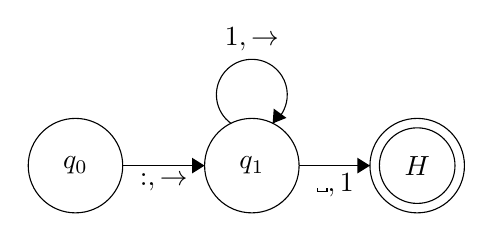
\begin{tikzpicture}[scale=0.2]
\tikzstyle{every node}+=[inner sep=0pt]
\draw [black] (3.3,-34.6) circle (3);
\draw (3.3,-34.6) node {$q_0$};
\draw [black] (14.5,-34.6) circle (3);
\draw (14.5,-34.6) node {$q_1$};
\draw [black] (25,-34.6) circle (3);
\draw (25,-34.6) node {$H$};
\draw [black] (25,-34.6) circle (2.4);
\draw [black] (6.3,-34.6) -- (11.5,-34.6);
\fill [black] (11.5,-34.6) -- (10.7,-34.1) -- (10.7,-35.1);
\draw (8.9,-35.1) node [below] {$:,\rightarrow$};
\draw [black] (17.5,-34.6) -- (22,-34.6);
\fill [black] (22,-34.6) -- (21.2,-34.1) -- (21.2,-35.1);
\draw (19.75,-35.1) node [below] {$\tvs,1$};
\draw [black] (13.177,-31.92) arc (234:-54:2.25);
\draw (14.5,-27.35) node [above] {$1,\rightarrow$};
\fill [black] (15.82,-31.92) -- (16.7,-31.57) -- (15.89,-30.98);
\end{tikzpicture}
\end{center}
\end{example}

\begin{example}[Unary addition of two natural numbers]
This machine uses the alphabet $\{1,*\}$ and correct input is of form $*,a*,*b,a*b$ followed by blanks  ($a$ and $b$ are strings containing only $1$). Here $a$ and $b$ represent the numbers to be added together in unary notation. Output is the unary number that is left on the tape when the machine accepts. 
\begin{center}
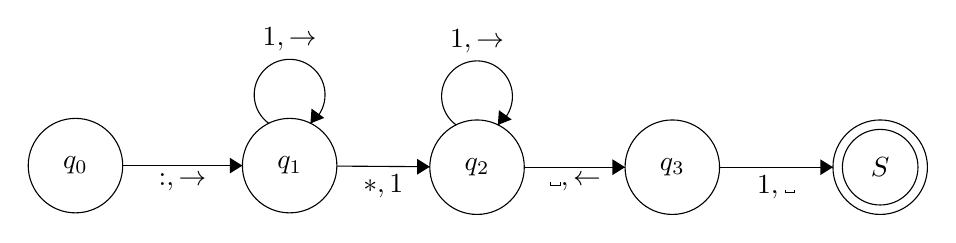
\begin{tikzpicture}[scale=0.2]
\tikzstyle{every node}+=[inner sep=0pt]
\draw [black] (10.5,-19.2) circle (3);
\draw (10.5,-19.2) node {$q_0$};
\draw [black] (24.1,-19.2) circle (3);
\draw (24.1,-19.2) node {$q_1$};
\draw [black] (36,-19.3) circle (3);
\draw (36,-19.3) node {$q_2$};
\draw [black] (48.4,-19.3) circle (3);
\draw (48.4,-19.3) node {$q_3$};
\draw [black] (61.6,-19.3) circle (3);
\draw (61.6,-19.3) node {$S$};
\draw [black] (61.6,-19.3) circle (2.4);
\draw [black] (13.5,-19.2) -- (21.1,-19.2);
\fill [black] (21.1,-19.2) -- (20.3,-18.7) -- (20.3,-19.7);
\draw (17.3,-19.7) node [below] {$:,\rightarrow$};
\draw [black] (27.1,-19.23) -- (33,-19.27);
\fill [black] (33,-19.27) -- (32.2,-18.77) -- (32.2,-19.77);
\draw (30.05,-19.76) node [below] {$*,1$};
\draw [black] (22.777,-16.52) arc (234:-54:2.25);
\draw (24.1,-11.95) node [above] {$1,\rightarrow$};
\fill [black] (25.42,-16.52) -- (26.3,-16.17) -- (25.49,-15.58);
\draw [black] (34.677,-16.62) arc (234:-54:2.25);
\draw (36,-12.05) node [above] {$1,\rightarrow$};
\fill [black] (37.32,-16.62) -- (38.2,-16.27) -- (37.39,-15.68);
\draw [black] (39,-19.3) -- (45.4,-19.3);
\fill [black] (45.4,-19.3) -- (44.6,-18.8) -- (44.6,-19.8);
\draw (42.2,-19.8) node [below] {$\tvs,\leftarrow$};
\draw [black] (51.4,-19.3) -- (58.6,-19.3);
\fill [black] (58.6,-19.3) -- (57.8,-18.8) -- (57.8,-19.8);
\draw (55,-19.8) node [below] {$1,\tvs$};
\end{tikzpicture}
\end{center}

Note that strictly speaking the $\delta$ represented by this diagram isn't a function. This is not a problem because all state/input combinations not on the diagram can be considered to map to an undrawn reject state, so the machine rejects if it gets input of an incorrect form. The machine is guaranteed (hopefully) to work correctly when the input has the correct form.

\end{example}



Because we demand that $\delta$ is a function, the only way a run of a TM can stop is by the machine entering one of the halt states. A run of a TM may not halt! 

\begin{exercise}
Design a Turing machine using the alphabet $\Sigma=\{0,1\}$ that does not halt for any input.
\end{exercise}



\subsection{Decision Problems}
Turing machines are important because they are closely related to a special kind of question called a \emph{decision problem}. Decision problems are things like
\begin{enumerate}
\item Given a graph $G$, is $G$ connected?
\item Does a given string of English characters contain the word \emph{biscuits} as a substring?
\item Is a given propositional formula satisfiable?
\item Is a given natural number prime?
\end{enumerate}

The answer to all these questions is either yes or no (depending on the graph/string etc. we are given). An answer always exists in theory, though we may not know how to find it. A decision problem has a generic component (the question), and a specific instance (the particular object we are asking the question about). For example, the generic component of the first question is whether a graph is connected, and the specific instance is whatever specific graph we are given. The generic component of the second question is whether a string contains the word \emph{biscuits}, and the specific instance is the particular string we are given. The result of applying the generic question to a specific instance will be either yes or no.

More abstractly a decision problem is a set of objects that can be partitioned into two, with one of the sets representing the objects for which the answer is \emph{yes}, and the other representing the objects for which the answer is \emph{no}. We usually say the set of all objects is the set of \emph{instances} of the problem, and that the two subsets partition the set of instances into \emph{yes instances} and \emph{no instances}. Looking again at our 2nd example, here the instance set is the set of all strings of English characters, the yes instances are those strings containing the word \emph{biscuits}, and the no instances are those not containing it. E.g. \emph{jhbybiscuitslp} is a yes instance, and \emph{bsjsppojlkn} is a no instance. 


\subsection{Formal Languages}
To connect Turing machines and decision problems we need to be able to represent decision problems in a formal language. That is we need to \emph{encode} the instances of the problem using the symbols from a finite alphabet. That is, we want to find an alphabet so that every instance of the problem is represented by a string of finite length, and distinct instances have distinct strings (abstractly we want a 1-1 map from the set of instances to the set of finite strings over some finite alphabet). Recall the following definitions and facts:
\begin{itemize}
\item A (finite) alphabet $\Sigma$ is a finite set of symbols, e.g. $\{a,b,c\}$,\\ or $\{0,1,2,3,4,5,6,7,8,9\}$.
\item A string over $\Sigma$ is a sequence of characters, e.g. 01001, or the digits of $\pi$.
\item The \emph{length} of a string is the number of characters it contains. Given a string $s$ we use $|s|$ to denote the length of $s$. E.g $|01001|=5$, and the length of the string defined by the digits of $\pi$ is $\omega$ (this symbol means countably infinite).
\item The string with no elements is called the \emph{empty string}. We denote it using $\epsilon$, and $|\epsilon|=0$ by definition.
\item If $a=a_1\ldots a_m$ and $b=b_1\ldots b_n$ are strings over the same alphabet then we can \emph{concatenate} them to get $ab=a_1\ldots a_m b_1\ldots b_n$. Note that $|ab|=|a|+|b|$.
\item For all strings $a$ we have $\epsilon a = a$, and for all finite length $a$ we have $a\epsilon=a$.
\item The set of all finite length strings over $\Sigma$ is denoted by $\Sigma^*$.
\item A \emph{formal language} over $\Sigma$ is a subset of $\Sigma^*$.
\item If $L$ is a formal language over $\Sigma$ then we can define the characteristic function of $L$ by $\chi_L:\Sigma^*\to\{0,1\}$ and $\chi_L(s) = \begin{cases}1 \text{ if } s\in L \\
0 \text{ if } s\notin L \end{cases}$   
\end{itemize}

\begin{definition}[encoding scheme]
If $\Sigma$ is a finite alphabet, $D$ is a decision problem, and $I_D$ is the set of all instances of $D$, an encoding scheme for $D$ using $\Sigma$ is a function $\mathbf{code}: I_D\to \Sigma^*$ such that:
\begin{enumerate}
\item if $x,y\in I_D$ and $x\neq y$ we must have $\mathbf{code}(x)\neq \mathbf{code}(y)$ (i.e. $\mathbf{code}$ is $1-1$),
\item it is possible to work out if a string in $\Sigma^*$ is $\mathbf{code}(x)$ for some $x\in I_D$, and 
\item the process for converting $x$ to $\mathbf{code}(x)$ and $\mathbf{code}(x)$ to $x$ is well defined. 
\end{enumerate}
\end{definition}

Using encoding we can turn decision problems into formal languages as follows.
\begin{definition}[$L_D$]\label{D:LD}
Given a decision problem $D$, a finite alphabet $\Sigma$, and an encoding for $D$ using $\Sigma$, the language defined by $D$ is the set $L_D=\{\textbf{code}(x):x$ is a yes instance of $D\}$.
\end{definition}

So, if we encode $D$ using $\Sigma$, the set $\Sigma^*$ will be partitioned into three subsets: the set of codes of the yes instances ($L_D$), the set of codes of the no instances, and the set of strings that are not the code of any instance of $D$. 

Definition \ref{D:LD} shows us how an encodable decision problem $D$ defines a formal language $L_D$, and the problem of deciding whether an instance of $D$ is `yes' or `no' is equivalent to the problem of deciding whether the code of that instance is in $L_D$ or not. This also works in reverse in the obvious way. Any formal language $L$ defines a decision problem $D_L$ of the form ``is this word from $\Sigma^*$ in $L$?". 


\subsection{Turing Machines and Decision Problems}
We can now discuss the relationship between Turing machines and decision problems. 

\begin{definition}[Decidable]\label{D:dec}
An (encodable) decision problem $D$ is decidable if there is a Turing machine $T$ that accepts when its input is the code of a yes instance of $D$, and rejects when its input is the code of a no instance (or not the code of an instance at all). We say $T$ decides $D$.
\end{definition}

The obvious question now is, ``Is every decision problem that can be encoded using a finite alphabet decidable?" Many people intuitively felt that the answer should be yes, but it turns out the answer is actually no. We will prove this later. Studying the kinds of decision problems that cannot be decided by a Turing machine is the focus of a large part of this course. For now we make another definition.

\begin{definition}[Semidecidable]\label{D:semidec}
An (encodable) decision problem $D$ is semidecidable if there is a Turing machine $T$ that accepts when its input is the code of a yes instance of $D$, and does not halt (i.e. it runs forever) when its input is the code of a no instance (or not the code of an instance at all). We say $T$ semidecides $D$.
\end{definition}  

It turns out that some encodable decision problems are not even semidecidable, and we also prove this later. We saw in the previous section that encodable decision problems are equivalent to formal languages, and there are versions of definitions \ref{D:dec} and \ref{D:semidec} that apply to languages.


\begin{exercise}
Prove that every decidable decision problem is also semidecidable.
\end{exercise}

\begin{definition}[Recursive]
A formal language $L$ over a finite alphabet $\Sigma$ is recursive if there is a Turing machine $T$ that takes input $x$ from $\Sigma^*$ and accepts when $x\in L$ and rejects when $x\notin L$.  
\end{definition}

\begin{definition}[Recursively enumerable]
A formal language $L$ over a finite alphabet $\Sigma$ is recursively enumerable if there is a Turing machine $T$ that takes input $x$ from $\Sigma^*$ and accepts when $x\in L$ and runs forever when $x\notin L$. We often shorten \emph{recursively enumerable} to \emph{r.e.}).  
\end{definition}

By definition of $L_D$ and $D_L$ we have the following correspondences for encodable decision problems:
\begin{align*}
D \text{ is decidable}&\iff L_D \text{ is recursive}\\
D_L \text{ is decidable}&\iff L \text{ is recursive}\\
D \text{ is semidecidable}&\iff L_D \text{ is recursively enumerable}\\
D_L \text{ is semidecidable}&\iff L \text{ is recursively enumerable}\\
\end{align*} 

\begin{example}[Palindromes]
Let $\Sigma=\{a,b\}$. This TM takes as input finite strings from $\Sigma^*$ and accepts if they are palindromes (i.e. if they are the same forwards and backwards ,e.g. $abbabba$), and rejects if they are not. I.e. it proves that the set of palindromes using $a$ and $b$ is recursive.

\begin{center}
\resizebox{\columnwidth}{!}{%
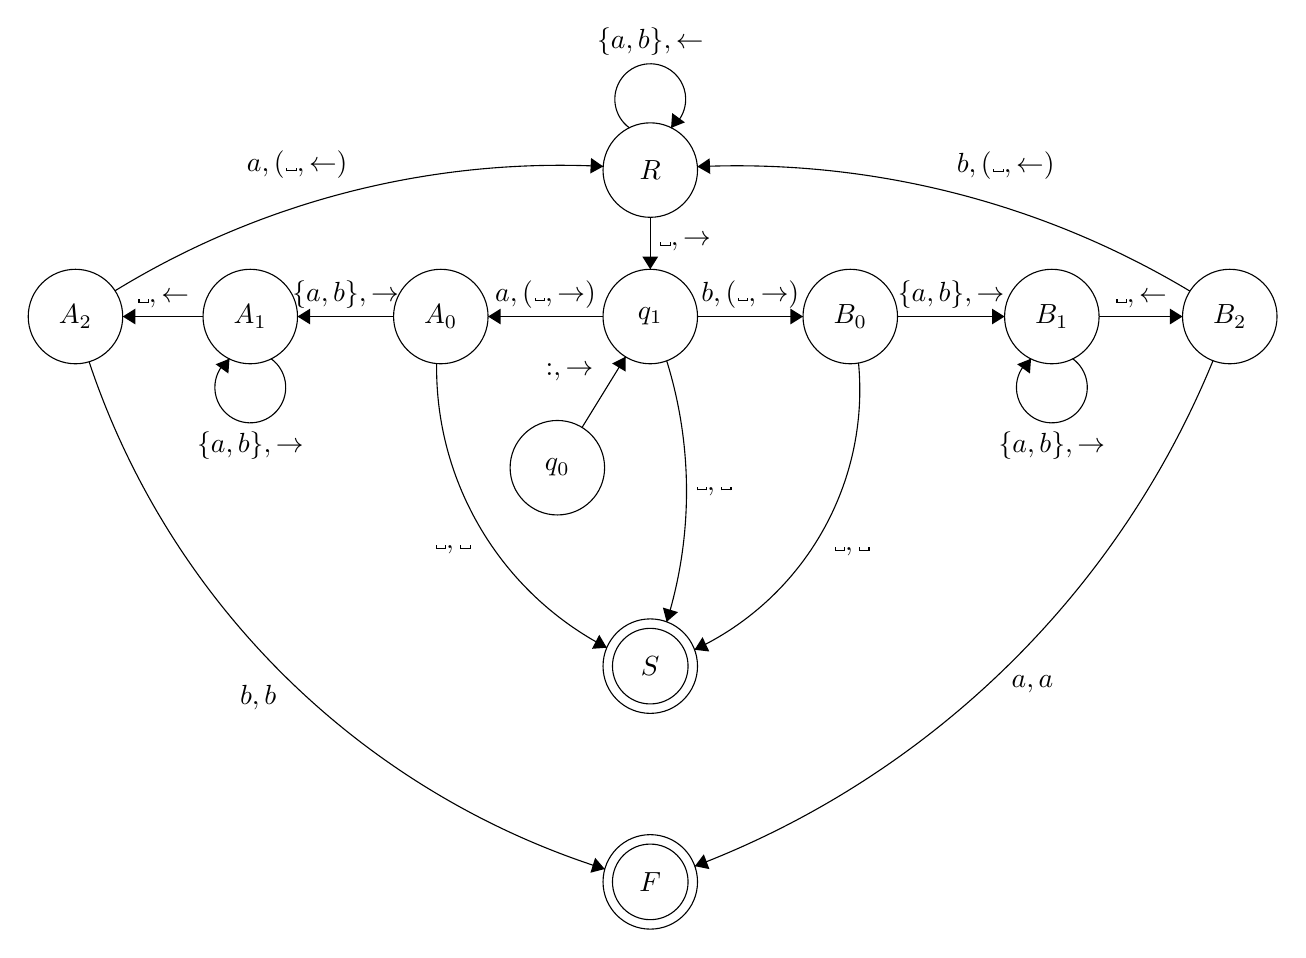
\begin{tikzpicture}[scale=0.2]
\tikzstyle{every node}+=[inner sep=0pt]
\draw [black] (39.6,-15.5) circle (3);
\draw (39.6,-15.5) node {$q_1$};
\draw [black] (52.3,-15.5) circle (3);
\draw (52.3,-15.5) node {$B_0$};
\draw [black] (65.1,-15.5) circle (3);
\draw (65.1,-15.5) node {$B_1$};
\draw [black] (76.4,-15.5) circle (3);
\draw (76.4,-15.5) node {$B_2$};
\draw [black] (26.3,-15.5) circle (3);
\draw (26.3,-15.5) node {$A_0$};
\draw [black] (14.2,-15.5) circle (3);
\draw (14.2,-15.5) node {$A_1$};
\draw [black] (3.1,-15.5) circle (3);
\draw (3.1,-15.5) node {$A_2$};
\draw [black] (33.7,-25.1) circle (3);
\draw (33.7,-25.1) node {$q_0$};
\draw [black] (39.6,-6.2) circle (3);
\draw (39.6,-6.2) node {$R$};
\draw [black] (39.6,-51.4) circle (3);
\draw (39.6,-51.4) node {$F$};
\draw [black] (39.6,-51.4) circle (2.4);
\draw [black] (39.6,-37.7) circle (3);
\draw (39.6,-37.7) node {$S$};
\draw [black] (39.6,-37.7) circle (2.4);
\draw [black] (42.6,-15.5) -- (49.3,-15.5);
\fill [black] (49.3,-15.5) -- (48.5,-15) -- (48.5,-16);
\draw (45.95,-15) node [above] {$b,(\tvs,\ra)$};
\draw [black] (55.3,-15.5) -- (62.1,-15.5);
\fill [black] (62.1,-15.5) -- (61.3,-15) -- (61.3,-16);
\draw (58.7,-15) node [above] {$\{a,b\},\ra$};
\draw [black] (68.1,-15.5) -- (73.4,-15.5);
\fill [black] (73.4,-15.5) -- (72.6,-15) -- (72.6,-16);
\draw (70.75,-15) node [above] {$\tvs,\la$};
\draw [black] (36.6,-15.5) -- (29.3,-15.5);
\fill [black] (29.3,-15.5) -- (30.1,-16) -- (30.1,-15);
\draw (32.95,-15) node [above] {$a,(\tvs,\ra)$};
\draw [black] (23.3,-15.5) -- (17.2,-15.5);
\fill [black] (17.2,-15.5) -- (18,-16) -- (18,-15);
\draw (20.25,-15) node [above] {$\{a,b\},\ra$};
\draw [black] (11.2,-15.5) -- (6.1,-15.5);
\fill [black] (6.1,-15.5) -- (6.9,-16) -- (6.9,-15);
\draw (8.65,-15) node [above] {$\tvs,\la$};
\draw [black] (35.27,-22.54) -- (38.03,-18.06);
\fill [black] (38.03,-18.06) -- (37.18,-18.48) -- (38.04,-19);
\draw (36.02,-19.02) node [left] {$:,\ra$};
\draw [black] (5.614,-13.863) arc (121.48441:87.10459:54.115);
\fill [black] (36.61,-5.97) -- (35.84,-5.43) -- (35.79,-6.42);
\draw (17.18,-6.76) node [above] {$a,(\tvs,\la)$};
\draw [black] (42.592,-5.984) arc (92.59079:59.04384:55.895);
\fill [black] (42.59,-5.98) -- (43.41,-6.45) -- (43.37,-5.45);
\draw (62.17,-6.81) node [above] {$b,(\tvs,\la)$};
\draw [black] (66.423,-18.18) arc (54:-234:2.25);
\draw (65.1,-22.75) node [below] {$\{a,b\},\ra$};
\fill [black] (63.78,-18.18) -- (62.9,-18.53) -- (63.71,-19.12);
\draw [black] (15.523,-18.18) arc (54:-234:2.25);
\draw (14.2,-22.75) node [below] {$\{a,b\},\ra$};
\fill [black] (12.88,-18.18) -- (12,-18.53) -- (12.81,-19.12);
\draw [black] (38.277,-3.52) arc (234:-54:2.25);
\draw (39.6,1.05) node [above] {$\{a,b\},\la$};
\fill [black] (40.92,-3.52) -- (41.8,-3.17) -- (40.99,-2.58);
\draw [black] (39.6,-9.2) -- (39.6,-12.5);
\fill [black] (39.6,-12.5) -- (40.1,-11.7) -- (39.1,-11.7);
\draw (40.1,-10.85) node [right] {$\tvs,\ra$};
\draw [black] (36.714,-50.583) arc (-107.5108:-161.53957:50.565);
\fill [black] (36.71,-50.58) -- (36.1,-49.87) -- (35.8,-50.82);
\draw (14.7,-38.89) node [below] {$b,b$};
\draw [black] (75.335,-18.304) arc (-22.28191:-69.13662:57.811);
\fill [black] (42.43,-50.4) -- (43.36,-50.59) -- (43,-49.65);
\draw (63.87,-38.25) node [below] {$a,a$};
\draw [black] (36.842,-36.526) arc (-117.36188:-180.78654:20.004);
\fill [black] (36.84,-36.53) -- (36.36,-35.71) -- (35.9,-36.6);
\draw (28.23,-30.3) node [left] {$\tvs,\tvs$};
\draw [black] (52.825,-18.45) arc (5.36879:-64.91413:18.221);
\fill [black] (42.41,-36.66) -- (43.35,-36.77) -- (42.92,-35.86);
\draw (51.16,-30.43) node [right] {$\tvs,\tvs$};
\draw [black] (40.643,-18.311) arc (17.27171:-17.27171:27.917);
\fill [black] (40.64,-34.89) -- (41.36,-34.27) -- (40.4,-33.98);
\draw (42.4,-26.6) node [right] {$\tvs,\tvs$};
\end{tikzpicture}
}
\end{center}

This TM introduces some new shorthand notation. The command `$a,(\tvs,\ra)$' for example signifies ``if reading $a$ write $\tvs$ then move the tape head right", and the command `$\{a,b\},\ra$' means ``if reading either $a$ or $b$ then move the tape head right.
\end{example}

\begin{exercise}
Let $\Sigma=\{1\}$, and let $L$ be the subset of $\Sigma^*$ containing all strings of even length. Prove that $L$ is recursive.
\end{exercise}


\subsection{Pushdown Automata}
As we have discussed, Turing machines are strictly more powerful than FSMs due to them effectively having infinite memory. This means there are tasks we can design a TM to perform that can not be done by an FSM. At this point we may be curious if there's a model of computation between FSMs and TMs. It turns out the answer is yes. A \emph{pushdown automaton} is another abstract computation system based on FSMs. Unlike an FSM, a pushdown automaton also has access to infinite memory in the form of a stack. In addition to reading input a pushdown automaton also has access to the top element of the stack, and its $\delta$ function takes this information into account. Pushdown automata not only change state but may also manipulate the stack. It turns out that this makes them strictly more powerful than FSMs, but strictly less powerful than Turing machines. However, pushdown automata with two stacks turn out to be equivalent to Turing machines, because we can use one stack to model the part of the tape to the left of the tape head, and the other to model the part of the tape to the right.    


\subsection{Computation and Language}
\begin{definition}[Recognize]
Let $M$ be an abstract machine capable of acting on input from $\Sigma^*$ for a finite alphabet $\Sigma$, and let $L\subseteq\Sigma^*$ be a language. We say $M$ recognizes $L$ if $M$ accepts on input $x$ if and only if $x\in L$. 
\end{definition}

According to this definition, every recursively enumerable language has a Turing machine that recognizes it (this is just the definition of r.e.). Moreover, every Turing machine $T$ defines a recursively enumerable language (just take the set of all $x$ such that $T(x)$ halts). This gives us a correspondence between the class of Turing machines and the class of r.e. languages.

\begin{theorem}
The class of recursively enumerable languages is precisely the class of languages that can be recognized by a Turing machine.
\end{theorem}

This is similar to the result that says that regular languages are precisely those that can be recognized by an FSM. Indeed, the connection between models of computation and formal languages is very strong, and we see this in the \emph{Chomsky hierarchy} (see figure \ref{F:chom}). The characterization of regular languages as those recognizable by an FSM, for example, gives us useful things like the \emph{pumping lemma} very easily (if you don't know what this is look it up!).

\begin{figure}[h]
\begin{center}
\begin{tabular}{ |c| c | }
 \hline \textbf{language} & \textbf{model of computation} \\ \hline
 recursively enumerable & Turing machines \\ \hline 
 context-sensitive & linear bounded automata \\ \hline
 context-free & pushdown automata \\ \hline
 regular & finite state machines\\ \hline
\end{tabular}
\end{center}
\caption{The Chomsky hierarchy of formal languages and their associated models of computation. Models of computation are arranged in order of power. On this course we are mainly interested in Turing machines. Note that it is possible to refine this hierarchy by adding extra classes, and this may result in something that is not linearly ordered.}
\label{F:chom}
\end{figure}



\end{document}